\documentclass[runningheads,10pt]{llncs}


% \usepackage[compact]{titlesec}
% \usepackage[margin=1.8cm]{geometry}
\usepackage{float}
\pagestyle{empty}

% \setlength{\parskip}{2pt}

\setlength{\parskip}{2pt}
\setlength{\floatsep}{4pt}
\setlength{\textfloatsep}{4pt}
\setlength{\intextsep}{4pt}
\setlength{\abovecaptionskip}{2pt}
\setlength{\belowcaptionskip}{0pt}

\usepackage[hidelinks]{hyperref}

\usepackage[T1]{fontenc}
\usepackage{graphicx}
\usepackage{amsmath}
\usepackage{amssymb}
\usepackage{booktabs}
\usepackage{array}
\usepackage{hyperref}
\usepackage{cite}
\usepackage{microtype}

\begin{document}

\title{\normalsize Analysis of Financial Market Dynamics using Neurocomputing for COVID-19 Regime Transitions}

\author{Dr.~N.~Ahana Priyanka\inst{1}\orcidID{0000-0002-8487-1043} \and
R.~Harishkanna\inst{2} \and
Dr.~R.~Sneka Nandhini\inst{3}}



\institute{Department of Computer Science and Engineering,\\
Sri Sivasubramaniya Nadar College of Engineering, Chennai, India\\
\email{ahanapriyankan@ssn.edu.in}, \email{harishkannar2312050@ssn.edu.in}}

\maketitle

%------------------------------------------------------------------
\vspace{-15pt}
\begin{abstract}
Financial markets are widely modeled as rational systems. However, practical evidence suggests that collective decision-making is influenced by interacting emotionally, risk-based, and control mechanisms. To capture this intricacy, this study introduces the Financial Connectome, a neuroscience-inspired pipeline that models the market as a collective cognitive network. This work investigates the long-standing disconnect between neuroscience and finance by mutually analyzing value, risk, sentiment, and control processes at the market level. Building on neurobiological theories of decision-making, a Neuro-Decision Systems (NDS) framework is suggested to examine the market dynamics reorganization under systemic stress. The framework is applied to 1,516 trading days of the NIFTY Bank Index spanning 2017--2023, encompassing the COVID-19 crisis period. The results indicate a significant structural reconfiguration of market states. The Neuro-Decision Score (NDS) exhibits a statistically significant post-COVID shift toward risk dominance, with Kolmogorov--Smirnov, permutation, and Mann--Whitney U tests all rejecting the null hypothesis ($p < 0.001$). In addition, average state persistence increases by approximately 24\%, indicating greater temporal rigidity in market dynamics. The ML-generalized NDS further strengthens the distributional separation, increasing the observed effect size from small to medium magnitude. Post-pandemic markets exhibit heightened sensitivity, reflected by higher activation frequencies across all cognitive systems. These findings suggest that market behavior undergoes measurable cognitive reorganization during periods of extreme uncertainty. The framework provides a structured approach for analyzing regime reconfiguration under sustained uncertainty.

\keywords{Neurofinance, COVID-19, Market, Decision system}
\end{abstract}

%------------------------------------------------------------------
\vspace{-15pt}
\section{Introduction}
\vspace{-10pt}
People often think of financial markets as rational systems in which prices reflect available information and agents act to maximize expected outcomes~\cite{lo2004}. This assumption provides a useful analytical foundation for the observed market behavior. Prices can swing wildly, things can change suddenly, and markets can stay out of balance for a long time, especially when there is a lot of uncertainty~\cite{hamilton1989}. These patterns indicate that market behavior is shaped not only by fundamentals but also by collective responses to risk and uncertainty~\cite{shiller2021,farmer2019}. The COVID-19 pandemic represents a global shock that disrupted economic activity and altered investor behavior across financial systems~\cite{baker2020,zaremba2021}. Unlike problems that do not last long, the pandemic brought constant uncertainty, repeated information shocks, and prolonged stress. This system gives a unique opportunity to study whether markets just take these hits and go back to the normal state, or whether such events indicate long-lasting changes in underlying decision dynamics.

Decision neuroscience shows that when people make choices, multiple cognitive systems are responsible for valuation, risk assessment, emotional processing, anomaly detection, and executive control~\cite{glimcher2014}. The relative influence of these systems varies with context, particularly under stress; when there is constant uncertainty, people get more sensitive to risk and less able to adapt~\cite{bach2012,coates2012}. Behavioral finance reflects these insights by documenting systematic deviations from rational behavior, including loss aversion, herding, and sentiment-driven pricing~\cite{kahneman1979,demartino2010}. However, most behavioral models focus on individual systems or aggregated outcomes, rarely addressing how decision processes interact and reorganize at the market level during crises.

Neurofinance seeks to bridge neuroscience with financial decision-making, yet existing studies are largely confined to laboratory experiments or small-scale datasets~\cite{boorman2009,alcaro2011}. Consequently, it remains unclear whether neuroscience-inspired decision frameworks can explain behavior in large, real-world financial markets with constant feedback, adaptation, and collective dynamics. Viewing the market as a collective decision system helps address this limitation. From this perspective, market behavior reflects the interaction of competing decision processes operating at scale, where changes in prices, volatility, and trading patterns correspond to shifts in the dominance of valuation, risk, sentiment, anomaly detection, and control processes~\cite{farmer2019}. This abstraction enables neuroscience-inspired concepts to be applied to large financial datasets without relying on individual-level neural measurements.

The COVID-19 crisis, therefore, serves as a natural experiment to test whether sustained uncertainty leads to lasting changes in collective market behavior. If markets function as adaptive decision systems, prolonged stress may increase risk sensitivity, reduce flexibility, and generate more persistent market regimes and altered equilibrium states, implying incomplete reversion to pre-crisis behavior~\cite{lo2004}.

Based on behavioral finance and neuroscientific evidence on stress and decision-making, three hypotheses are tested. First, post-crisis markets are expected to exhibit higher activation across decision processes related to risk~\cite{coates2012}. Second, market regimes are expected to become more persistent, with slower transitions between states~\cite{hamilton1989}. Third, markets are expected to stabilize around a risk-dominant equilibrium rather than reverting to pre-COVID-19 crisis conditions~\cite{kahneman1979}.

To test these hypotheses, the study employs a neuro-computational framework that integrates financial indicators with machine learning models to infer system activation states~\cite{gu2020,baker2020}. Financial time-series data are transformed into signals representing the competing decision processes, enabling the identification of regime transitions and structural shifts. The analysis was drawn from 1,516 trading days of the NIFTY Bank Index spanning both the pre-COVID and post-COVID time periods. Unlike traditional regime-switching models that focus on prices or volatility~\cite{hamilton1989}, the proposed framework finds the underlying decision dynamics observed in market behavior. A direct empirical comparison with Hidden Markov Models or other Markov-switching frameworks is reserved for future work to evaluate incremental explanatory value.

This study contributes to the literature in three ways. A neuroscience-inspired framework is introduced to model financial markets as interacting decision systems rather than purely rational mechanisms~\cite{kahneman1979}. Empirical evidence is provided that the COVID-19 crisis induced persistent changes in market decision dynamics. Increased rigidity and stronger risk dominance are observed in post-pandemic markets, indicating a long-lasting shift in collective behavior.

%------------------------------------------------------------------
\vspace{-10pt}
\section{Methodology}
% \vspace{-10pt}
\subsection{Data Description and Preprocessing}

Daily market observations of the NIFTY Bank Index covering 1,516 trading days are used in the empirical analysis. The data was divided into two regime periods: a Pre-COVID period from January 2017 to March 2020, comprising 773 trading days, and a Post-COVID period from April 2020 to February 2023, comprising 743 trading days. The NIFTY Bank Index is selected due to its high liquidity and strong sensitivity to macroeconomic and financial conditions, making it a suitable proxy for collective risk perception in the market sentiment of the Indian financial system. Raw price and volume data are processed to construct engineered market features that capture multiple dimensions of market behavior. Standard preprocessing techniques were implemented, which include forward-filling gaps in the data and discarding early observations caused by rolling-window calculations~\cite{hamilton1989}. Rolling volatility metrics, momentum indicators, and moving averages are computed using fixed window lengths to capture short-term and medium-term trends. To reduce the effect of outliers, specific features are winsorized. Feature normalization is done separately for the Pre-COVID and Post-COVID periods using zero-mean, unit-variance standardization~\cite{gu2020}, to prevent information leakage between time periods while maintaining local statistical structure.
\vspace{-10pt}
\subsection{Feature Construction}

A total of 22 engineered features are constructed across price, return, momentum, volatility, and volume dimensions~\cite{gu2020,farmer2019}. These features serve as observable representations of market activity and form the input space for subsequent modeling. The complete set of engineered features is summarized in Table~\ref{tab:features}. The feature set is designed to reflect both normal market behavior and stress-driven conditions. Trend and momentum indicators capture gradual changes in market direction, while volatility and abnormal trading measures capture sudden shocks. This structure enables the model to detect regime changes that are not visible from prices alone.

% Add \small before each tabular, e.g.:
\small
\begin{table}[ht]
\caption{Engineered Market Features}\label{tab:features}
\centering
\begin{tabular}{ll}
\toprule
\textbf{Category} & \textbf{Features} \\
\midrule
Price \& Returns & Open, High, Low, Close, Daily, Weekly, Monthly Returns \\
Momentum \& Trend & Momentum (30d), RSI, Index Strength, SMA (20/50/200), \\
                  & Price/MA50, Price/MA200, Above MA50, Above MA200 \\
Volatility \& Risk & Volatility (20d), Gap Open, Intraday Range \\
Volume            & Volume, Volume Spike \\
\bottomrule
\end{tabular}
\end{table}
\vspace{-10pt}
\subsection{Neurocomputational Framework}

Market behavior is interpreted through a neurocomputational framework inspired by decision neuroscience~\cite{glimcher2014,bach2012}. The market is not a single rational system; it is driven by human-brain-like decision processes. The proposed NDS framework conceptually examines dynamics as the interaction of distinct decision systems. Five decision systems corresponding to valuation, risk sensitivity, sentiment, social influence, anomaly detection, and executive control are examined~\cite{boorman2009,demartino2010}. The conceptual mapping to brain regions and functional roles is summarized in Table~\ref{tab:framework}. This mapping serves as a structural analogy to organize collective market dynamics and does not imply direct neuroscientific measurement.
% Add \small before each tabular, e.g.:
\small
\begin{table}[ht]
\caption{Five-System Neurocomputational Framework}\label{tab:framework}
\centering
\begin{tabular}{lll}
\toprule
\textbf{System} & \textbf{Region} & \textbf{Function} \\
\midrule
Value            & vmPFC    & Greed / Opportunity (Reward seeking) \\
Risk             & Amygdala & Fear / Safety (Threat detection) \\
Sentiment        & dmPFC    & Herd Mentality (Social following) \\
Anomaly Detection & Insula  & Gut Feeling (Abnormality sensing) \\
Control          & dlPFC    & Strategy (Signal filtering) \\
\bottomrule
\end{tabular}
\end{table}
\vspace{-15pt}
\subsection{System Activation Logic}
% \vspace{-10pt}
The study infers the activation state of each decision system using rule-based criteria applied to engineered market features. Market behavior is translated into binary ($0$ or $1$) activation states indicating whether a given system is active on a particular trading day~\cite{lo2004,kahneman1979}. Activation logic is summarized in Table~\ref{tab:activation}. These activation rules are designed to remain interpretable while consistent with financial intuition and neuroscientific motivation. A dominant mode of collective decision-making is reflected in each activation system rather than an isolated price movement. These rule-based criteria serve as transparent supervisory anchors rather than exhaustive representations of market dynamics. Fixed thresholds establish interpretable activation boundaries, but they may introduce rigidity and sensitivity to local fluctuations. The subsequent machine learning layer is therefore introduced to provide nonlinear generalization and interaction modeling beyond strict cutoff logic. The classifier does not change activation standards; instead, it learns decision boundaries that are smoother and approximate the rule-based working descriptions.
% Add \small before each tabular, e.g.:
\small
\begin{table}[ht]
\caption{Interpretable Threshold Criteria for System Activation}\label{tab:activation}
\centering
\begin{tabular}{ll}
\toprule
\textbf{System} & \textbf{Threshold Conditions} \\
\midrule
Value (vmPFC)      & RSI ($>65$ or $<35$), Momentum ($>0.8\sigma$), or Daily Return ($>1\sigma$) \\
Risk (Amygdala)    & Volatility ($>$ Median $+ 0.5\sigma$) or Extreme Loss ($< -1\sigma$) \\
Sentiment (dmPFC)  & Price deviation from MA-50 ($>2\%$) or MA-200 \\
Anomaly Detection  & Gap Open ($>1\sigma$), Intraday Range ($>$ Median $+ 0.5\sigma$), \\
                   & or Volume Spike ($>1.3\times$) \\
Control (dlPFC)    & Activation of two or more other systems \\
\bottomrule
\end{tabular}
\end{table}

The above criteria provide interpretable operational definitions of activation states, which are used as supervised targets in the classification framework.
% \vspace{-10pt}
\subsection{Neuro-Computational System Architecture}
% \vspace{-10pt}
The proposed Neuro-Financial Computing Framework is structured as a four-stage computational pipeline, illustrated in Fig.~\ref{fig:pipeline}. Raw market data is turned into interpretable neuro-decision signals while timeline structure and market condition context are preserved.

In the first stage, the \textit{Data Ingestion Layer} processes observations of the NIFTY Bank Index spanning 1,516 trading days. The framework treats the Pre-COVID and Post-COVID periods as distinct diagnostic regimes, enabling the analysis of structural changes in market decision dynamics without imposing artificial continuity across the crisis boundary.

In the second stage, the \textit{Neuro-Financial Computing Layer} transforms raw data into engineered financial features described earlier. These feature indicators represent underlying cognitive processes: momentum-based indicators capture reward-seeking behavior, volatility reflects threat sensitivity, and deviation-based indicators highlight stress-driven market conditions. This stage converts noisy observations into structured neuro-computational inputs.

The third stage, the \textit{Classification Layer}, functions as a set of computational ``neural scanners.'' Five independent XGBoost classifiers are employed, each corresponding to a decision system in the framework~\cite{chen2016}. For each trading day, the classifiers predict binary activation states from the engineered feature set. The model adopts a non-linear ensemble structure to capture the evolving and non-linear dynamics of market conditions~\cite{farmer2019}.

The final stage is the \textit{Evaluation Layer}, where system-level outputs are aggregated into decision metrics. The Neuro-Decision Score (NDS) is the primary output and evaluates regime rigidity and flexibility using persistence metrics, providing support for the proposed ``Vigilant Guard'' hypothesis.

\begin{figure}[h]
\centering
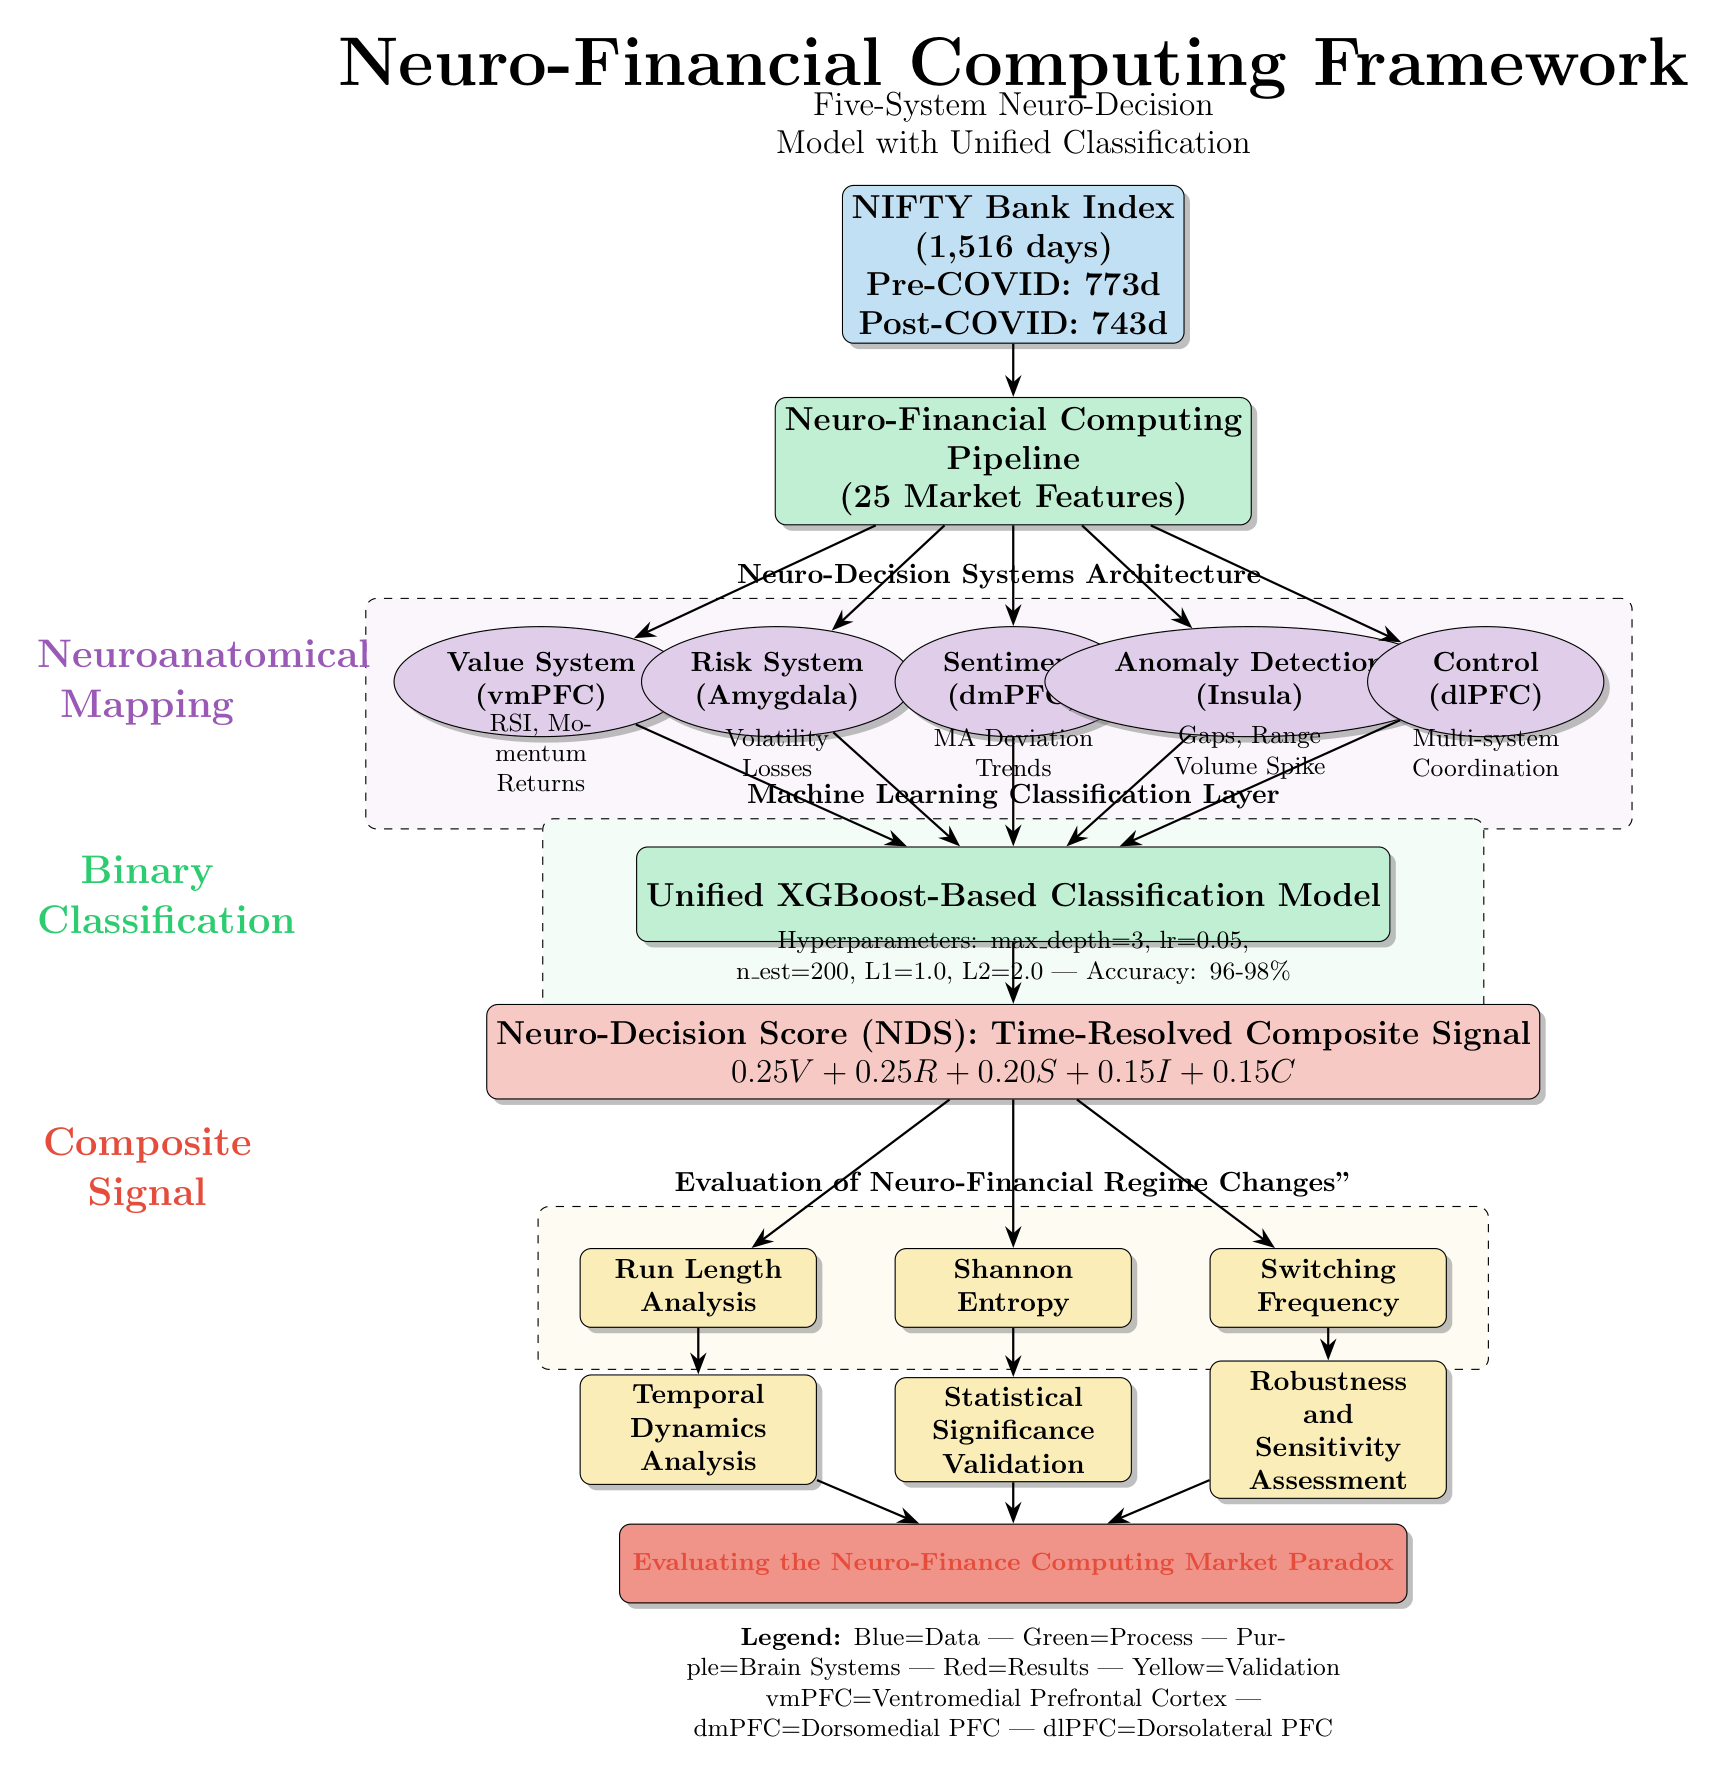
\includegraphics[width=0.6\textwidth]{architecture_diagram.png}
\caption{Neuro-Financial Computing Framework. The pipeline processes raw market data, maps engineered features to five brain systems using XGBoost classifiers, and aggregates signals into a Neuro-Decision Score.}
\label{fig:pipeline}
\end{figure}

\vspace{-15pt}
\subsection{Neuro-Financial Computing Model and Data Splits}
% \vspace{-10pt}
A separate XGBoost classifier is trained for each decision-making system to predict activation states using a set of features. A random 70/30 partition was employed for classification evaluation, and feature normalization was performed using training-set statistics to avoid information leakage~\cite{gu2020}. All models are trained with the same set of hyperparameters across all systems: maximum tree depth of 3, learning rate of 0.05, 200 estimators, L1 regularization of 1.0, L2 regularization of 2.0, and a subsample ratio of 0.8. Hyperparameters were fixed using conservative regularization principles, and no automated grid search was conducted. This ensures structural consistency across subsystems and prioritizes generalization over aggressive in-sample optimization. Using the same hyperparameters helps to compare the decision systems and avoids overfitting. Alternative models, including LightGBM and logistic regression, were evaluated, but XGBoost provided the most stable balance between accuracy and generalization and was therefore selected as the primary model.
\vspace{-15pt}
\subsection{Neuro-Decision Metrics}
\vspace{-10pt}
The Neuro-Decision Score (NDS) summarizes how the market makes decisions collectively. It is computed with the following formula:

\begin{equation}
\text{NDS}_t = \sum_{s} w_s \cdot A_{s,t}
\label{eq:nds}
\end{equation}

where $A_{s,t} \in \{0, 1\}$ denotes the activation state of system $s$ at time $t$. Systems such as Value, Sentiment, and Control carry positive weights. Systems associated with risk avoidance, such as Risk and Anomaly, carry negative weights. The final score gives a continuous measure of the prevailing balance between market value-dominant and risk-dominant states~\cite{glimcher2014,boorman2009}.

Alongside the NDS, market behavior is characterized using persistence and flexibility measurements. Run length indicates how often a pattern stays active. Switching frequency counts how often the market changes states. Entropy values were normalized by the maximum possible entropy to ensure comparability across regimes with differing sample sizes. Together, these metrics indicate whether the market remains adaptive or settles into rigid, stress-driven regimes~\cite{farmer2019}.

%------------------------------------------------------------------
\vspace{-15pt}
\section{Results}
% \vspace{-10pt}
\subsection{Validation of Inferred Activation State Classification}
\vspace{-5pt}
The framework checks whether the method for finding inferred activation states is valid before examining how the market changes. Five XGBoost classifiers are trained to detect market states related to Value, Risk, Sentiment, Anomaly Detection, and Control systems. All classifiers achieve strong predictive performance, with training accuracies over 98\% and test accuracies ranging from 96.05\% to 98.25\%. ROC--AUC values were consistently high (0.977--0.997), as shown in Table~\ref{tab:performance}, indicating robust separability between active and inactive states for each system. These results show that the classifiers reliably capture stable inferred activation states, which is essential for analyzing subsequent temporal and regime analyses.
\small
\begin{table}[ht]
\caption{XGBoost Classifier Performance}\label{tab:performance}
\centering
\begin{tabular}{llll}
\toprule
\textbf{System} & \textbf{Train Accuracy} & \textbf{Test Accuracy} & \textbf{ROC AUC} \\
\midrule
Value            & 98.632\% & 96.053\% & 0.992 \\
Risk             & 99.000\% & 96.053\% & 0.997 \\
Sentiment        & 98.906\% & 98.246\% & 0.993 \\
Anomaly Detection & 97.906\% & 96.491\% & 0.981 \\
Control          & 98.775\% & 96.053\% & 0.981 \\
\bottomrule
\end{tabular}
\end{table}
\vspace{-10pt}
\subsection{Differential Activation of Market Systems Pre- and Post-COVID}

To examine changes in market activity following the COVID-19 shock, the analysis compares activation frequencies of all systems between the Pre- and Post-COVID periods. Figure~\ref{fig:activation} shows the proportion of time each system remained active. All systems record higher activation levels in the Post-COVID period. The Risk system shows the largest increase, indicating greater awareness of adverse signals and uncertain conditions. The Value system also increased, reflecting more focus on spotting opportunities. Overall, Post-COVID markets display elevated multi-system activation across various decision-making processes.
\vspace{-6pt}
\begin{figure}[H]
\centering
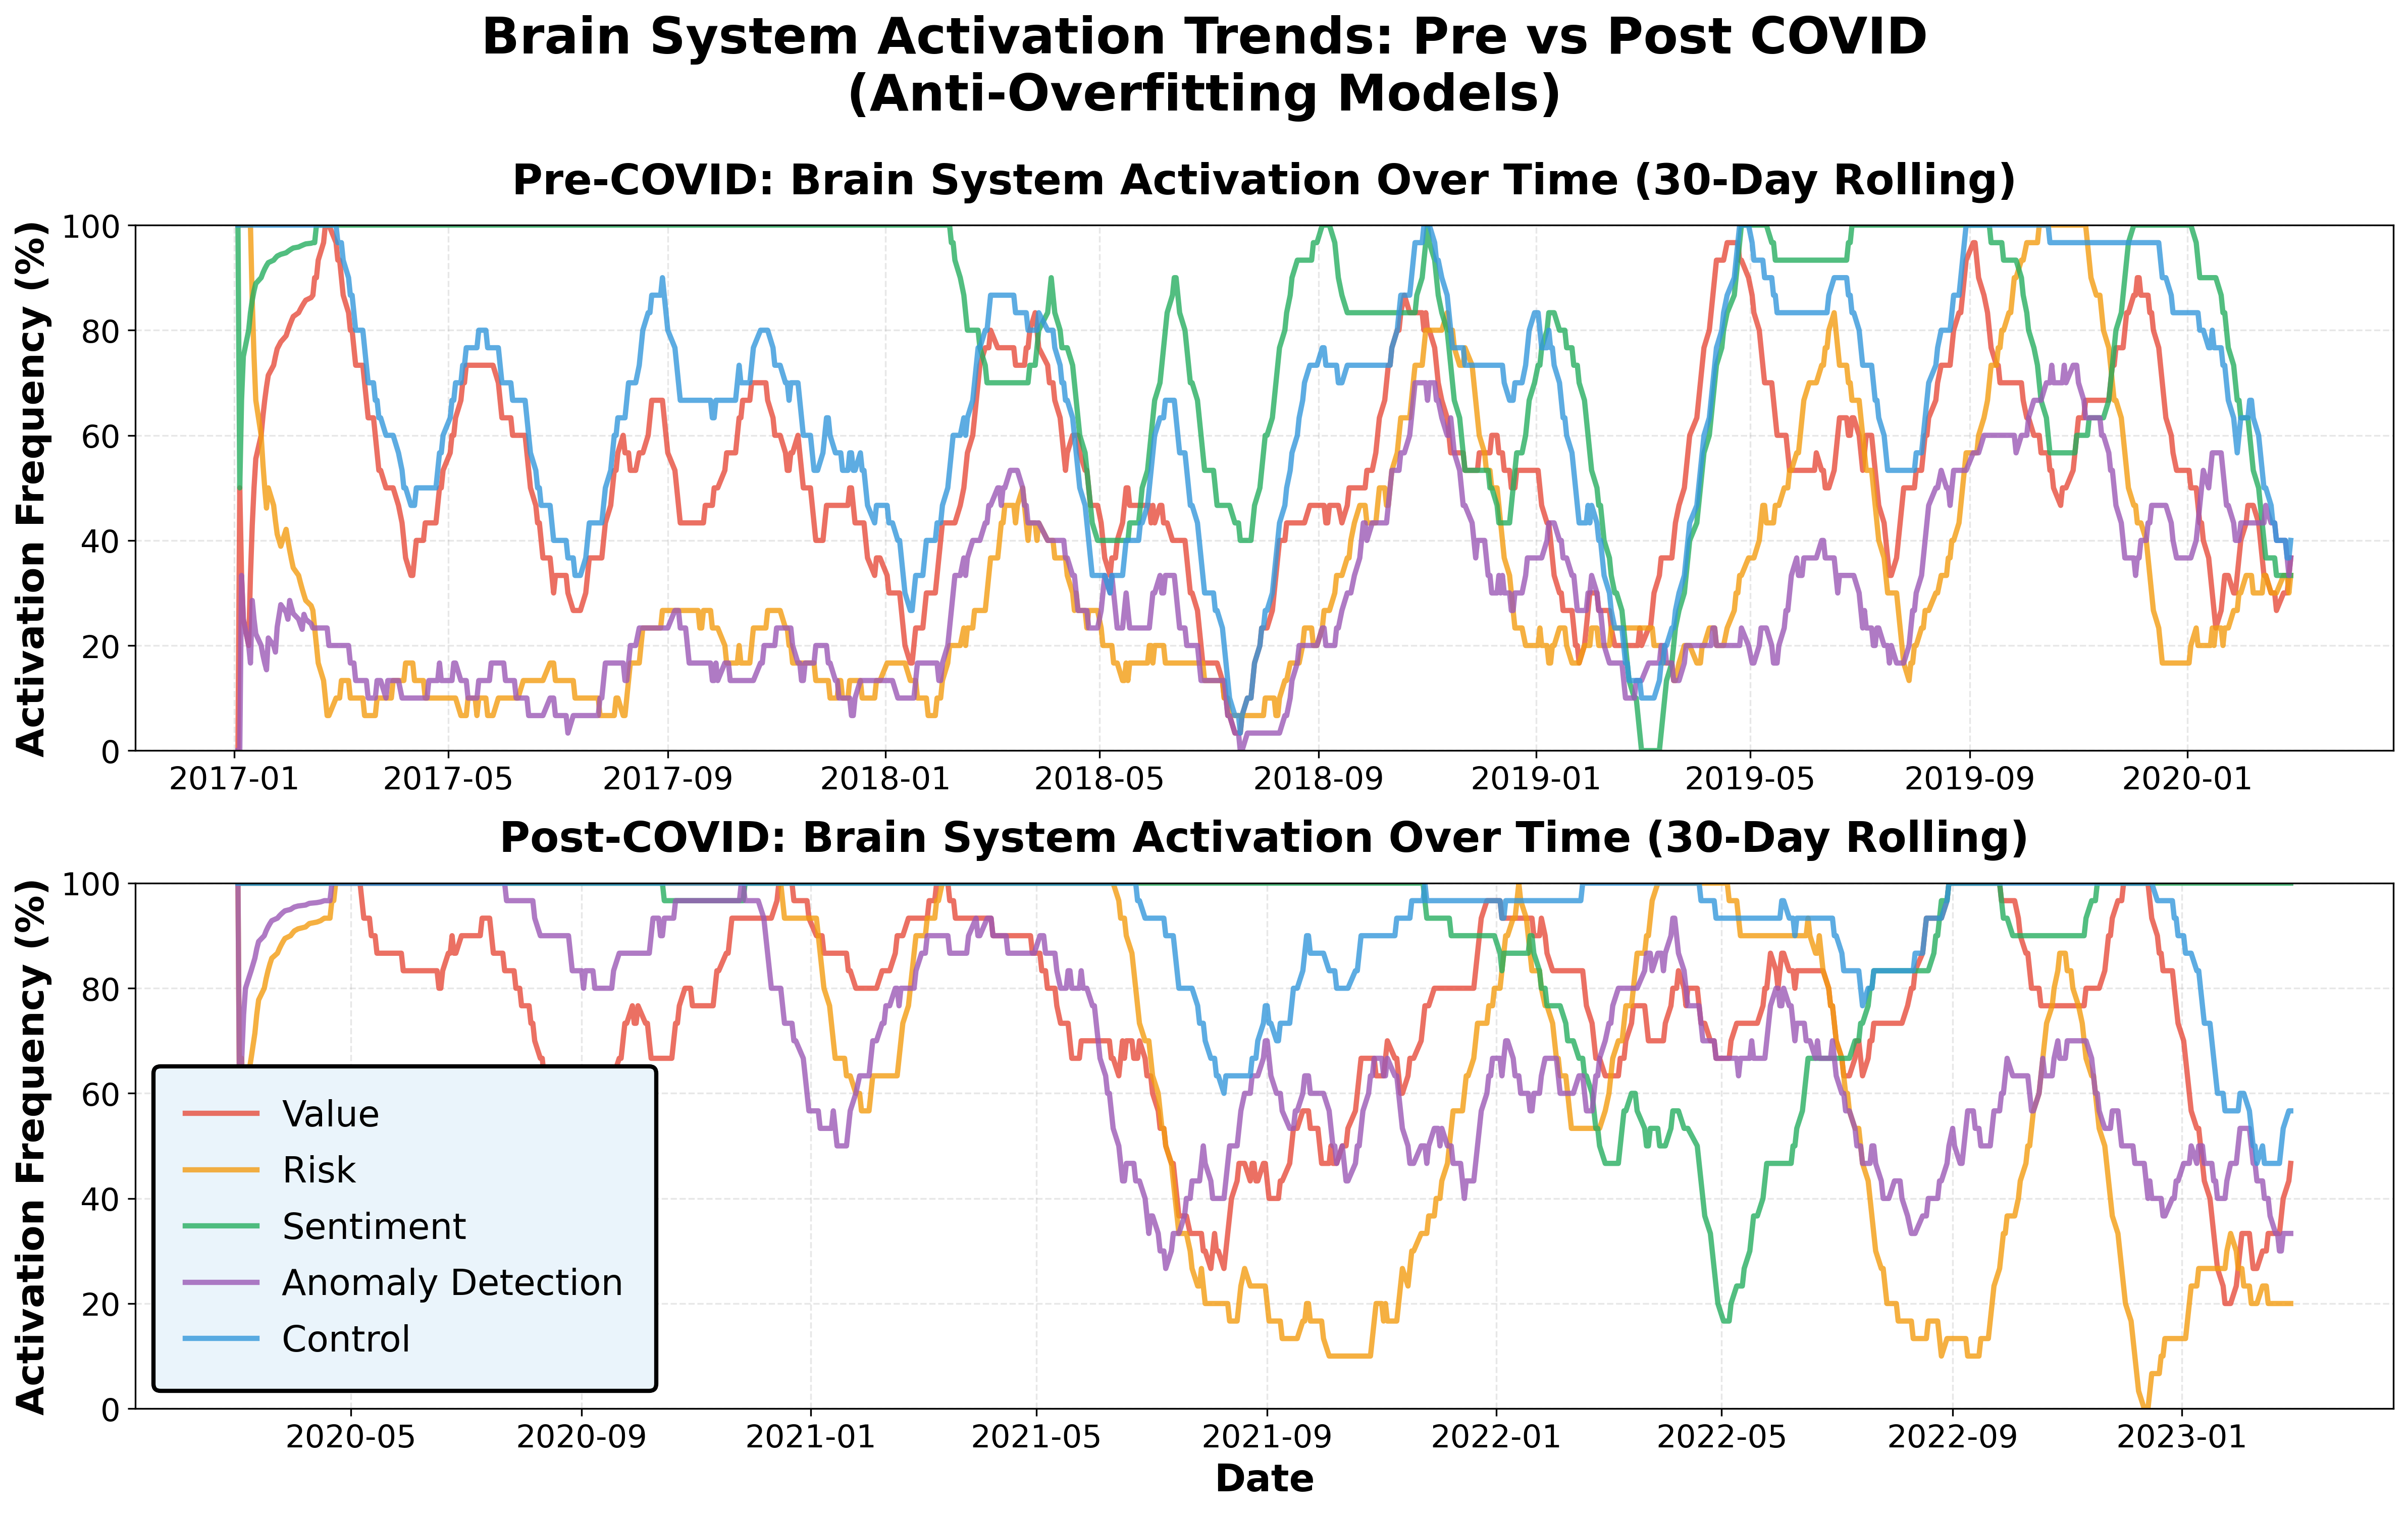
\includegraphics[width=0.6\textwidth]{activation_timeseries_combined.png}
\vspace{-4pt}
\caption{Brain system activation frequencies. The market became significantly more active Post-COVID (red), with the Risk system showing the most dramatic increase in firing rate.}
\label{fig:activation}
\end{figure}
\vspace{-20pt}
\subsection{Cross-System Synchronization and Collective Dynamics}
% \vspace{-10pt}

Beyond individual system behavior, collective dynamics are examined by analyzing cumulative system activations. The cumulative activation patterns for all systems are illustrated in Figure~\ref{fig:cumulative}. In the pre-COVID period, the activation curves were spread apart, indicating that different systems were dominant at different times. After COVID-19, the curves become steeper and cluster more closely together, indicating that the systems were firing simultaneously and remaining active. This pattern indicates that market systems began to act together more and lost independent behavior.

\begin{figure}[H]
\centering
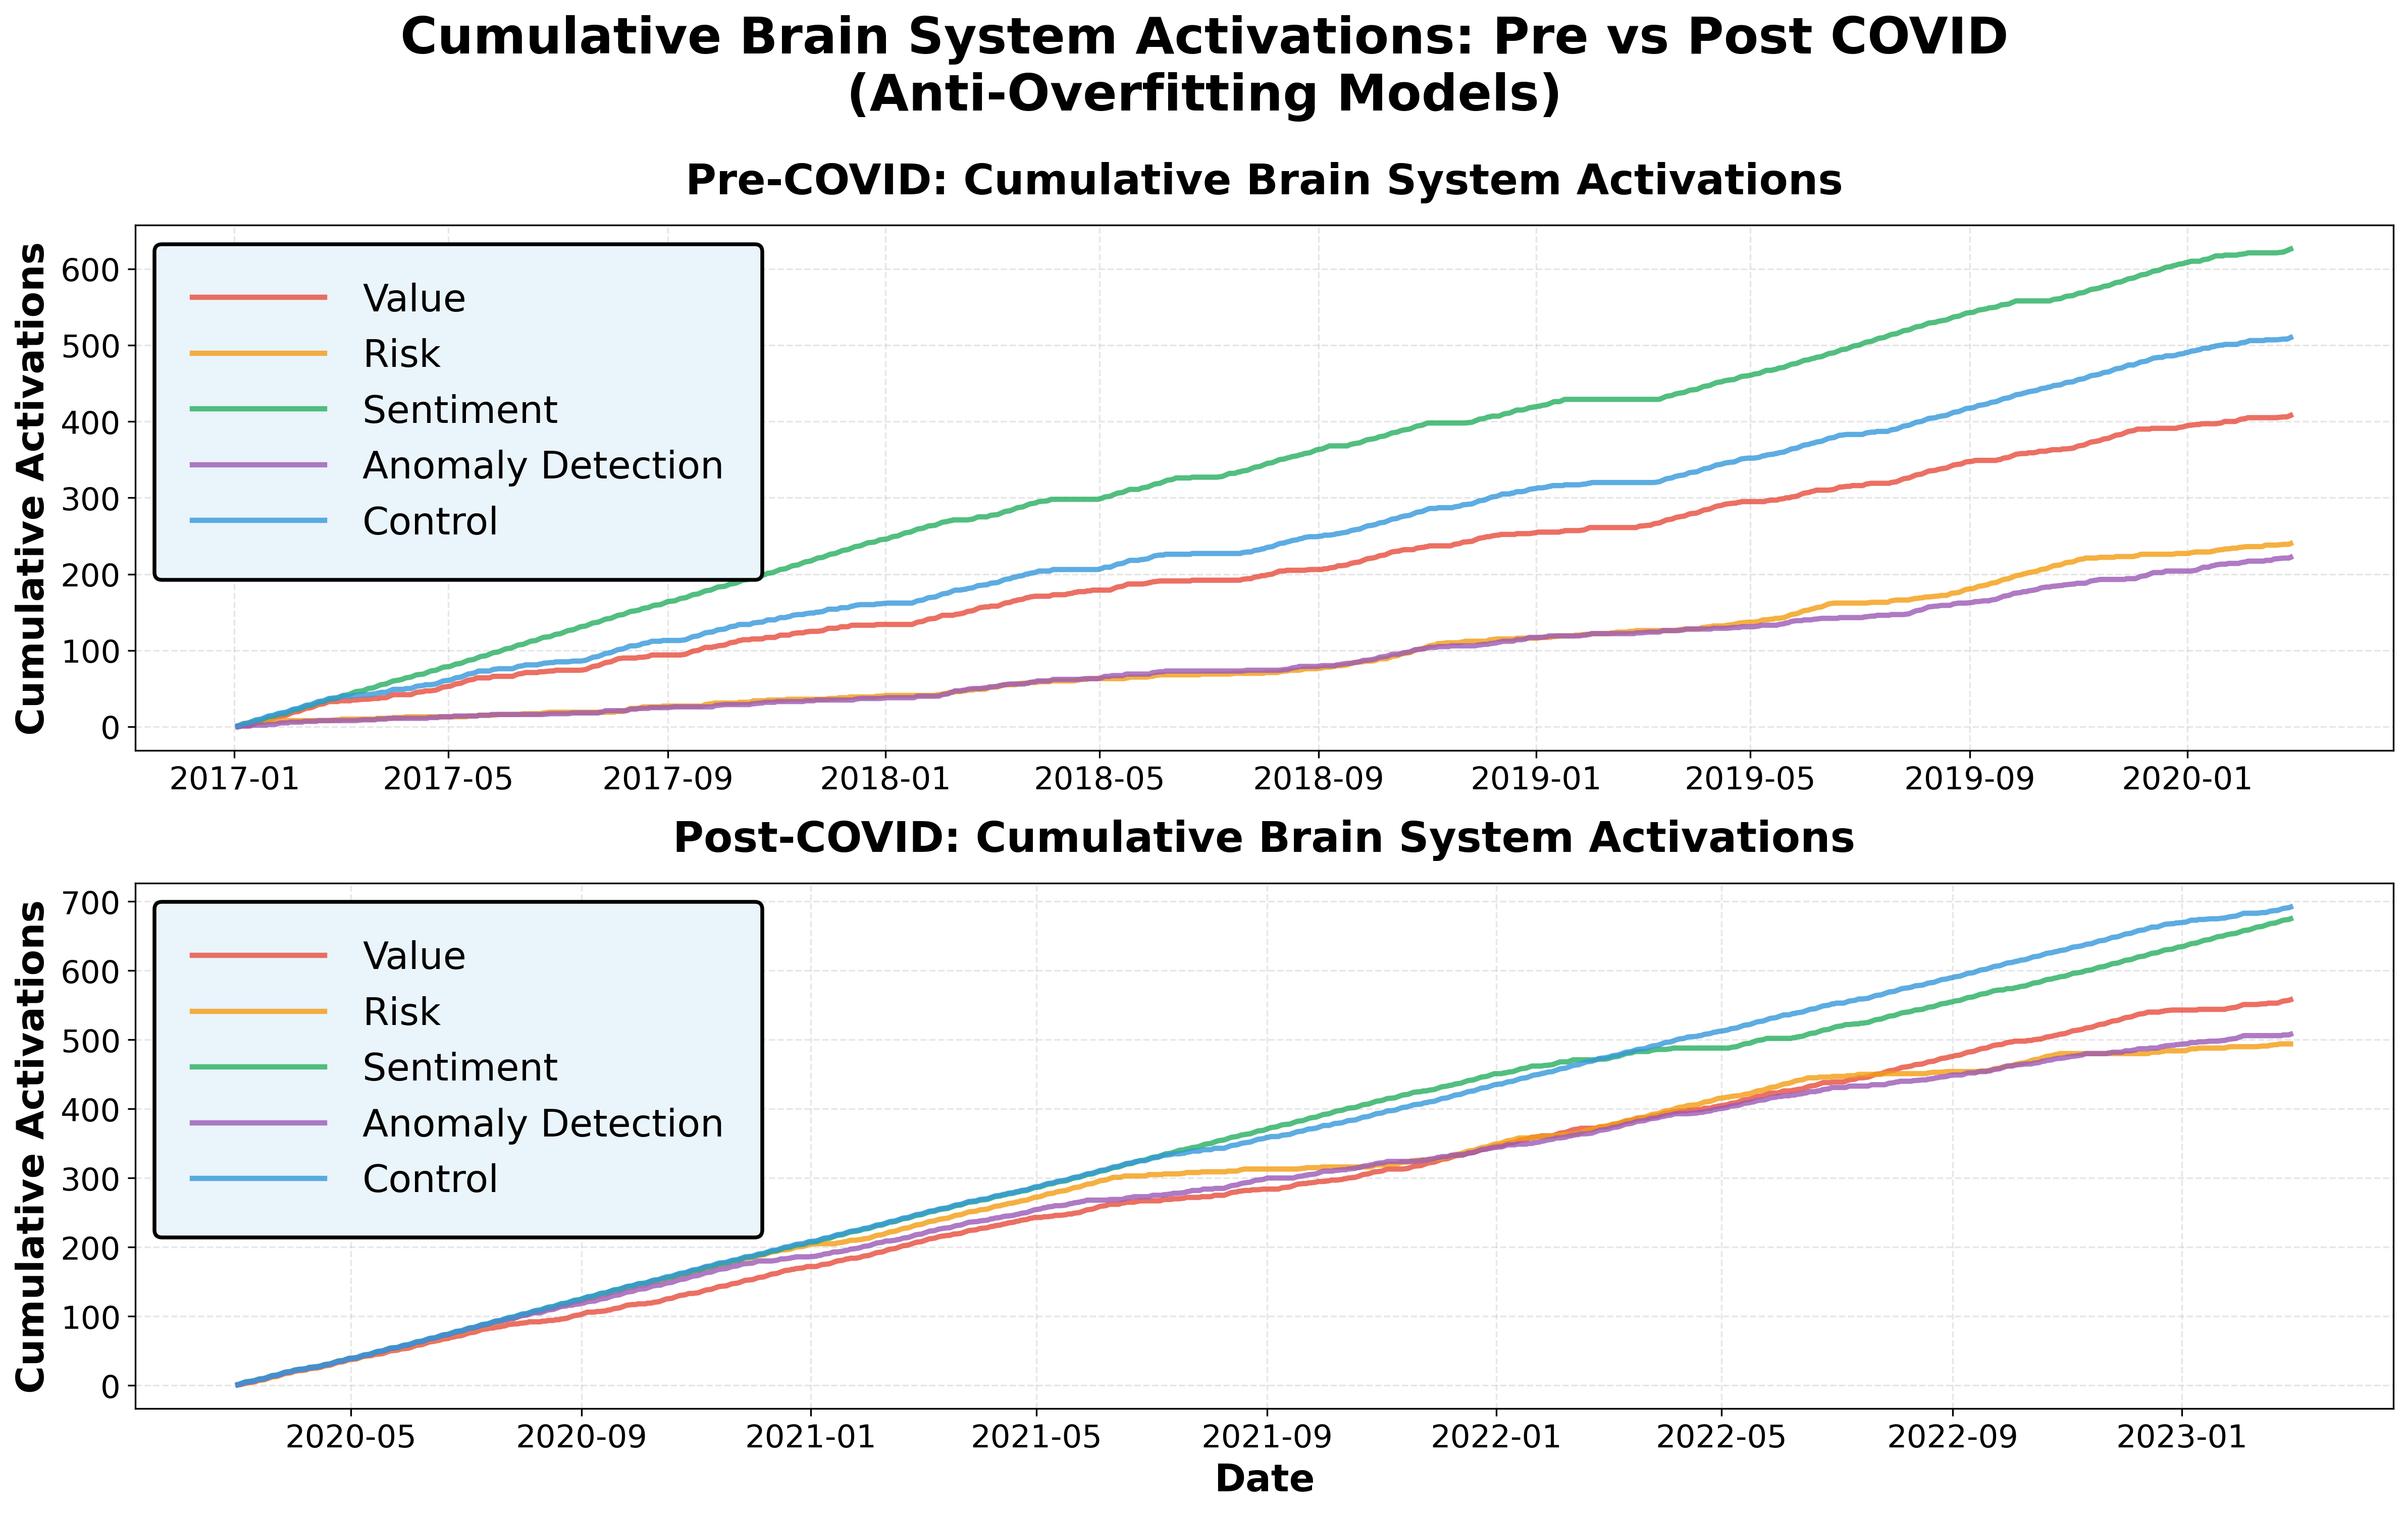
\includegraphics[width=0.6\textwidth]{activation_cumulative.png}
\caption{Cumulative Activations (``The Race''). Post-COVID, all systems accelerate and cluster together, indicating synchronized hyperactivity.}
\label{fig:cumulative}
\end{figure}
\vspace{-20pt}
\subsection{Distributional Shift in Neuro-Decision Score (NDS)}
\vspace{-15pt}
The analysis evaluates changes in the balance between risk- and value-dominant states using the Neuro-Decision Score (NDS). Figure~\ref{fig:nds} compares the NDS distributions before and after COVID-19. The Pre-COVID distribution remains narrow and centered near zero, indicating a relatively balanced market state. In the Post-COVID period, the distribution shifts toward negative values and widens, reflecting stronger dominance of risk-related states and elevated uncertainty. A Kolmogorov--Smirnov test confirms a statistically significant distributional difference between regimes ($D = 0.2464$, $p < 0.001$). A permutation test further indicates a significant decline in mean NDS ($\Delta = -2.01$, $p < 0.001$; Cohen's $d = -0.544$). Together, these results confirm that the observed shift reflects structural regime reconfiguration rather than sampling variability.

\begin{figure}[H]
\centering
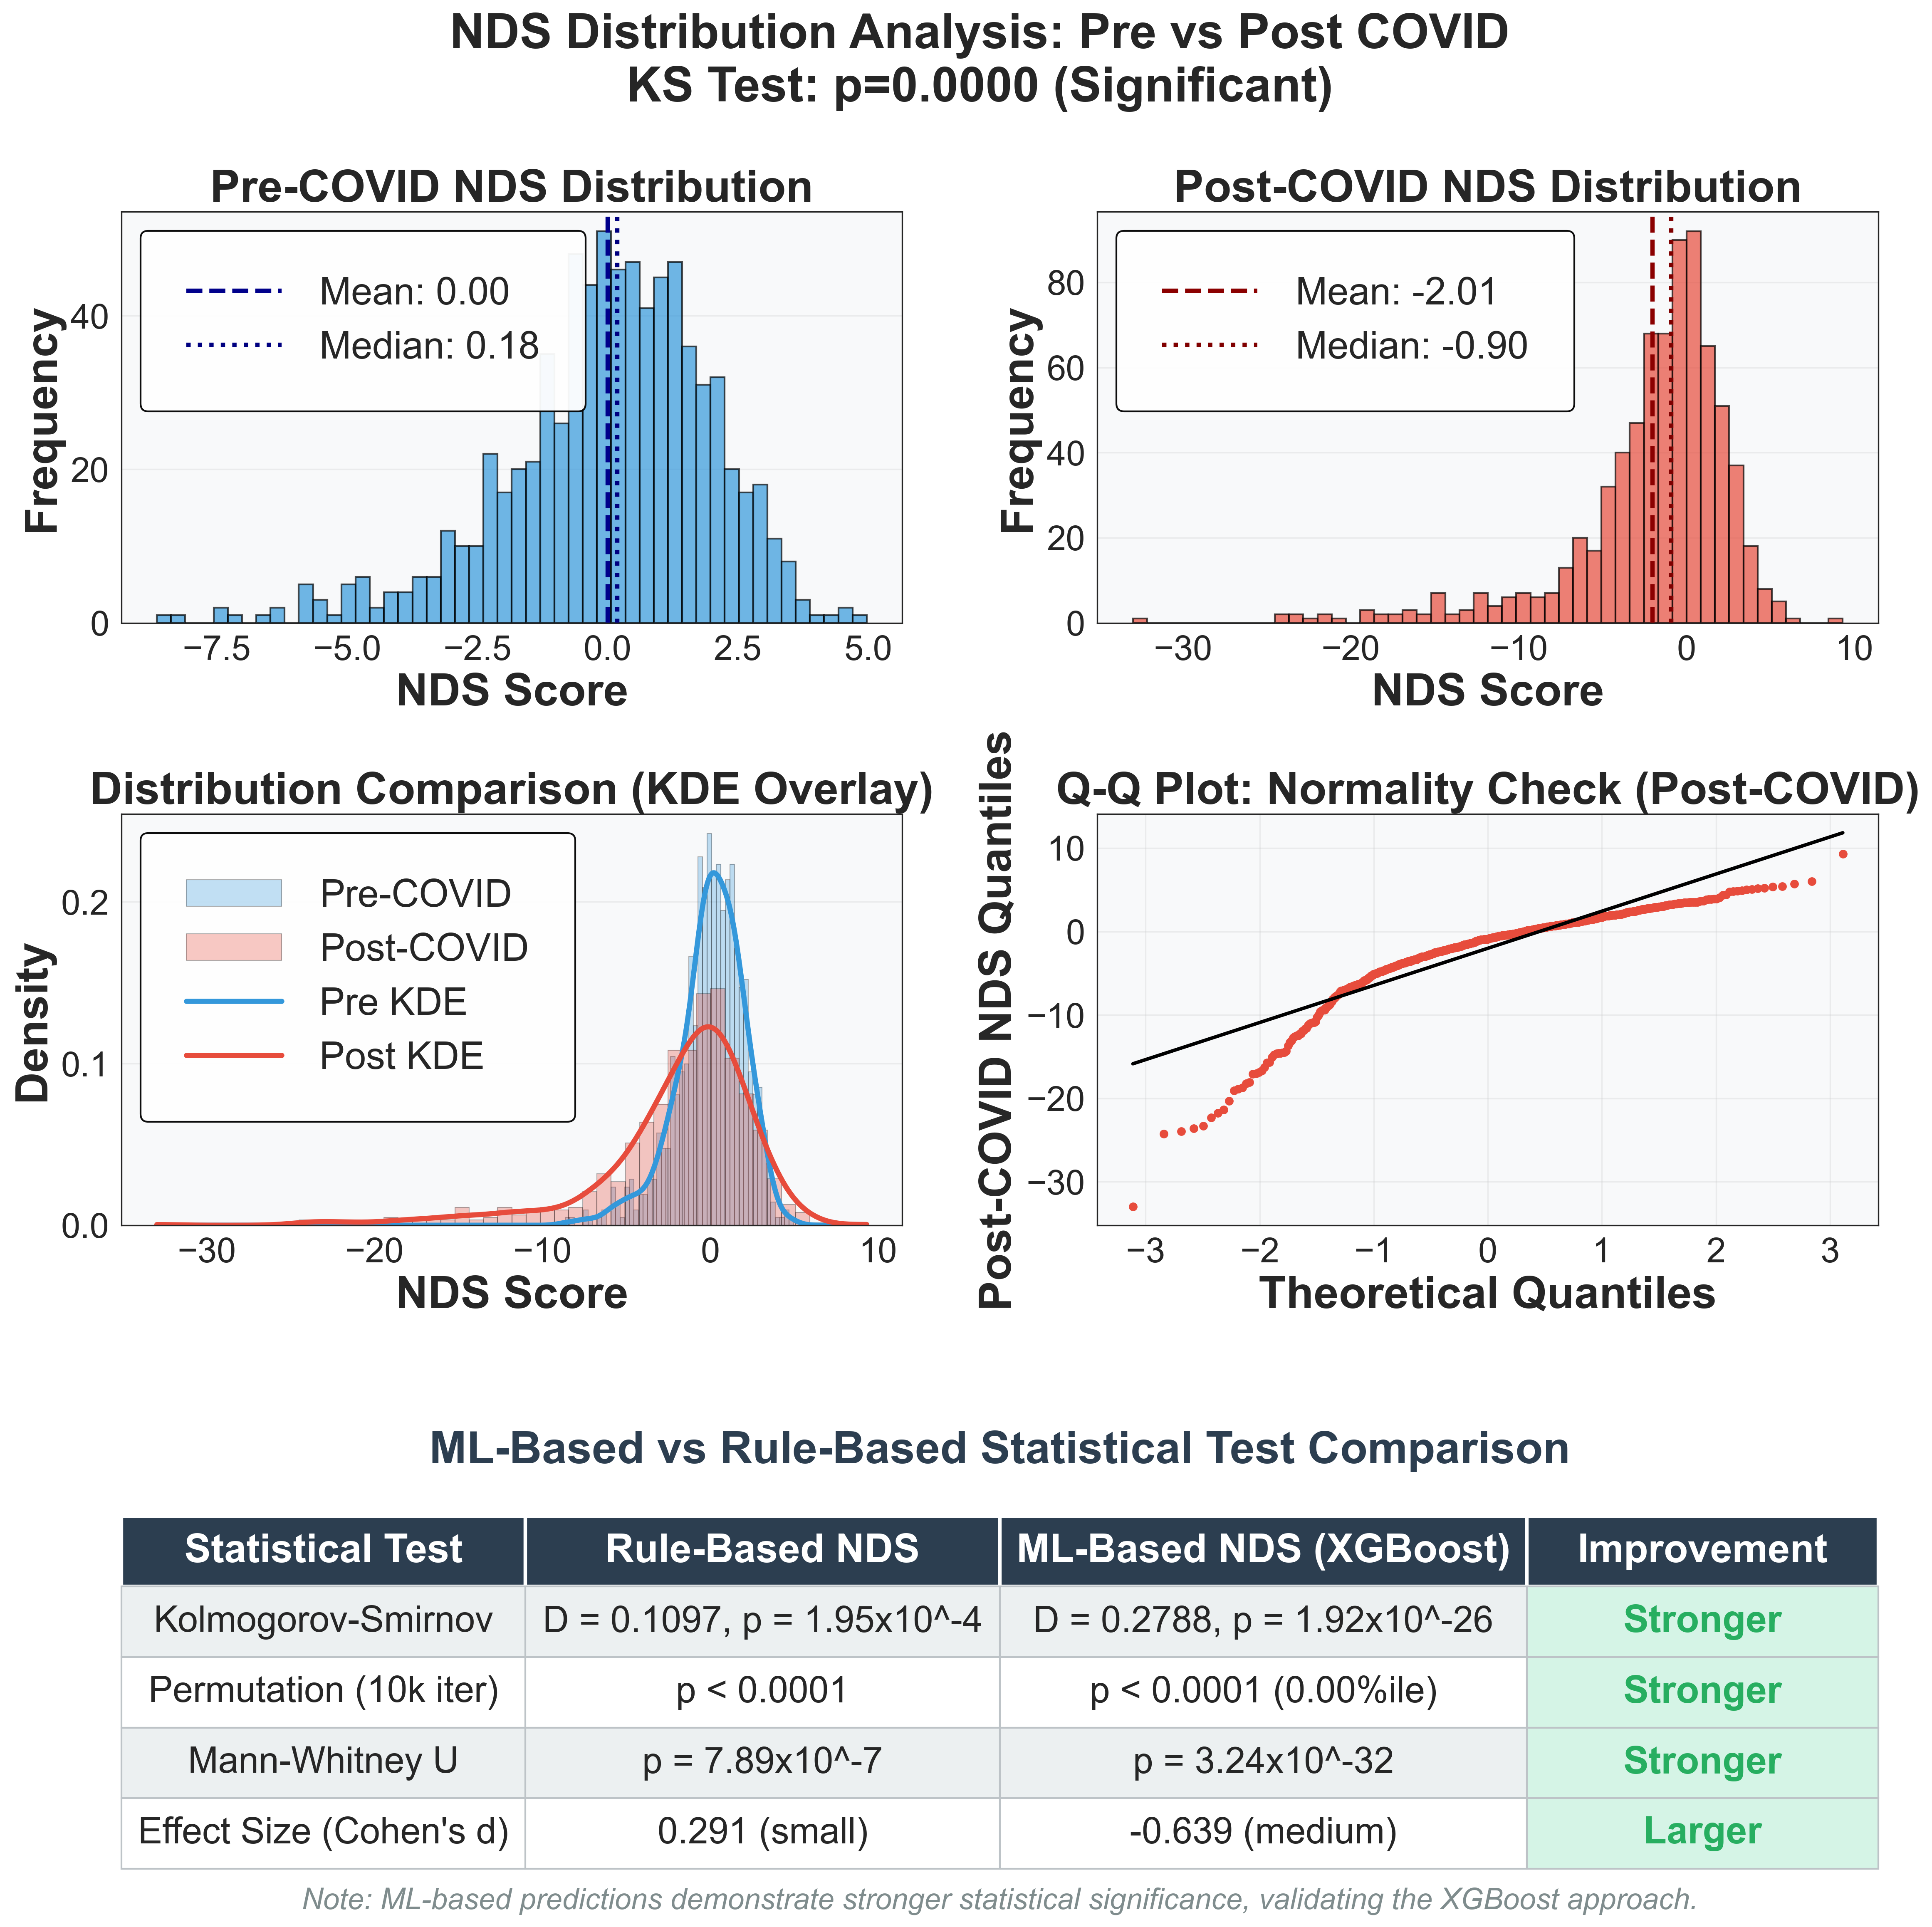
\includegraphics[width=0.5\textwidth]{nds_distribution_comparison.png}
\caption{NDS distribution before and after COVID-19. Post-COVID (red) shifts left relative to Pre-COVID (blue), indicating risk dominance (KS test, $p < 0.001$).}
\label{fig:nds}
\end{figure}
\vspace{-10pt}
\subsection{Changes in State Persistence Across Market Systems}

Temporal rigidity is assessed using the run length of continuous system activations. Run-length statistics across the Pre- and Post-COVID periods are compared in Figure~\ref{fig:persistence}(a). On average, run length increased by approximately 24\% across systems in the Post-COVID period. However, individual system-level Mann--Whitney U tests did not reach statistical significance, likely due to high variance in persistence durations. These results indicate that longer activation durations are maintained after COVID-19 once systems become active. As a complementary measure of temporal dynamics, system switching frequency was examined. Figure~\ref{fig:persistence}(b) presents the average number of state transitions for each system. In the Post-COVID period, switching frequency declines consistently across all systems. This reduction indicates diminished temporal flexibility and increased rigidity, supporting the conclusion that market dynamics became more rigid following the shock.

\begin{figure}[H]
\centering
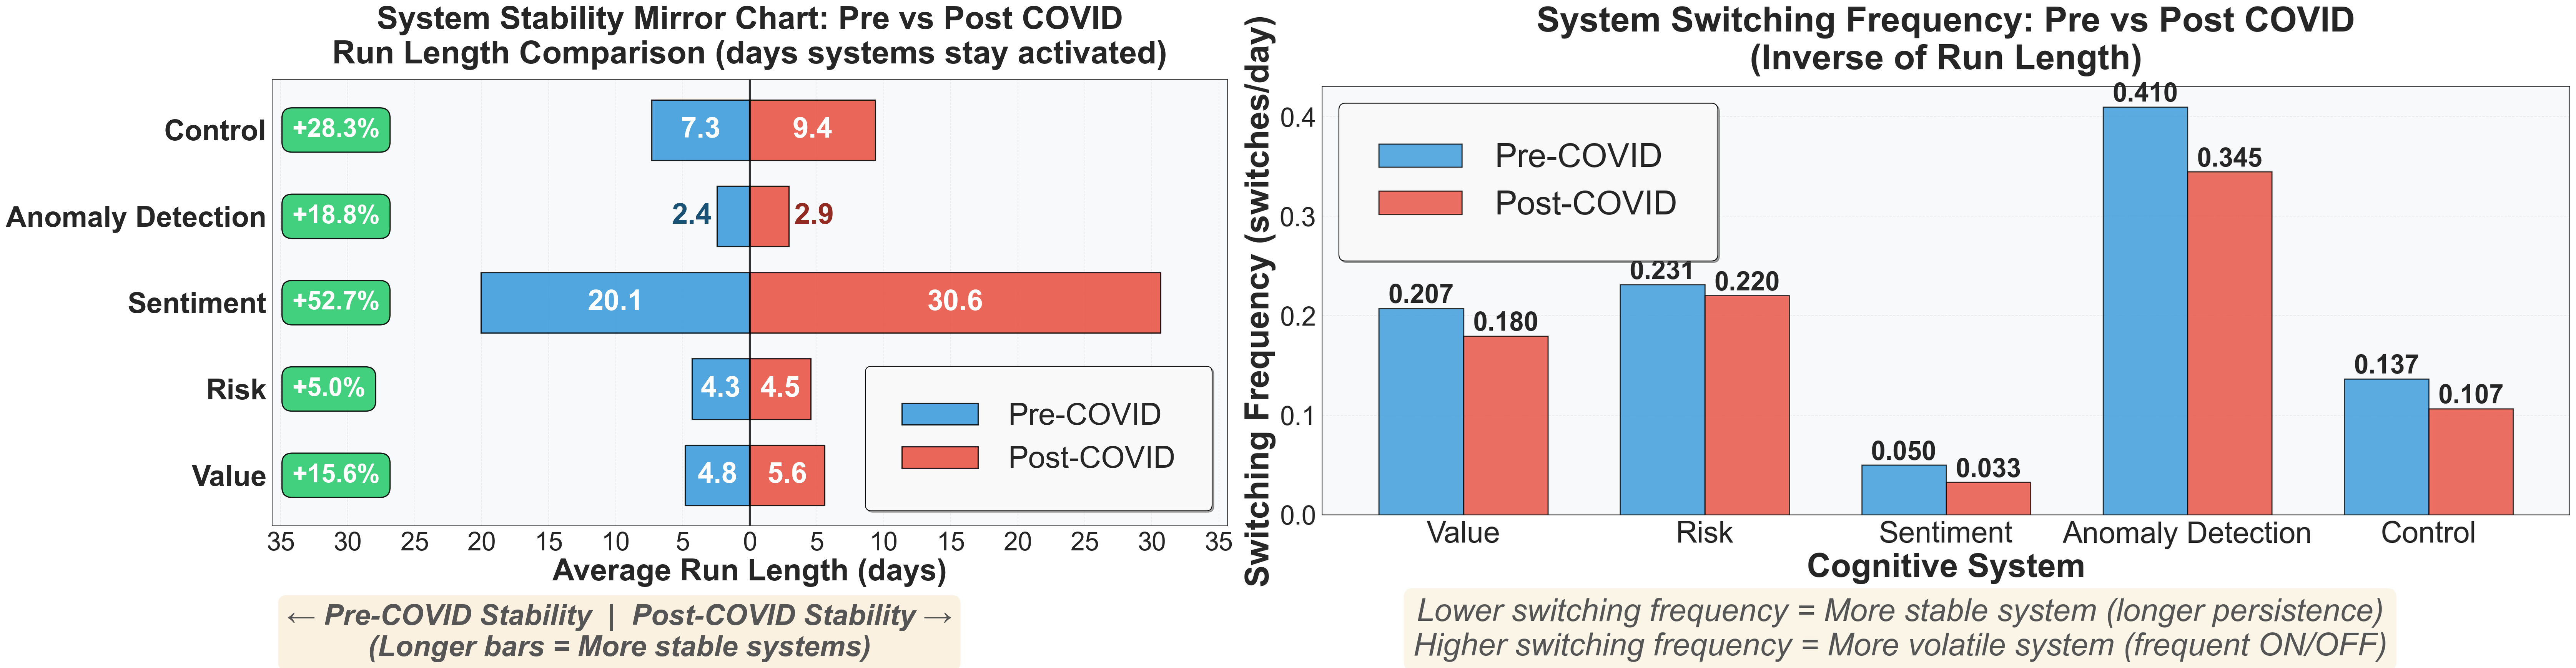
\includegraphics[width=0.8\textwidth]{combined_side_by_side.png}
\caption{(a) Run length mirror chart showing increased post-COVID persistence of market states. (b) Switching frequency comparison indicating reduced transitions and increased rigidity in the post-COVID period.}
\label{fig:persistence}
\end{figure}
\vspace{-10pt}
\subsection{Post-COVID Market Regime Characterization}

Integrating activation frequency, persistence, synchronization, and NDS analyses reveals a distinct post-COVID market regime. As illustrated in Figure~\ref{fig:paradox}, higher stability in system persistence is observed alongside sustained risk dominance and increased uncertainty in the Post-COVID market.
\begin{figure}[H]
\centering
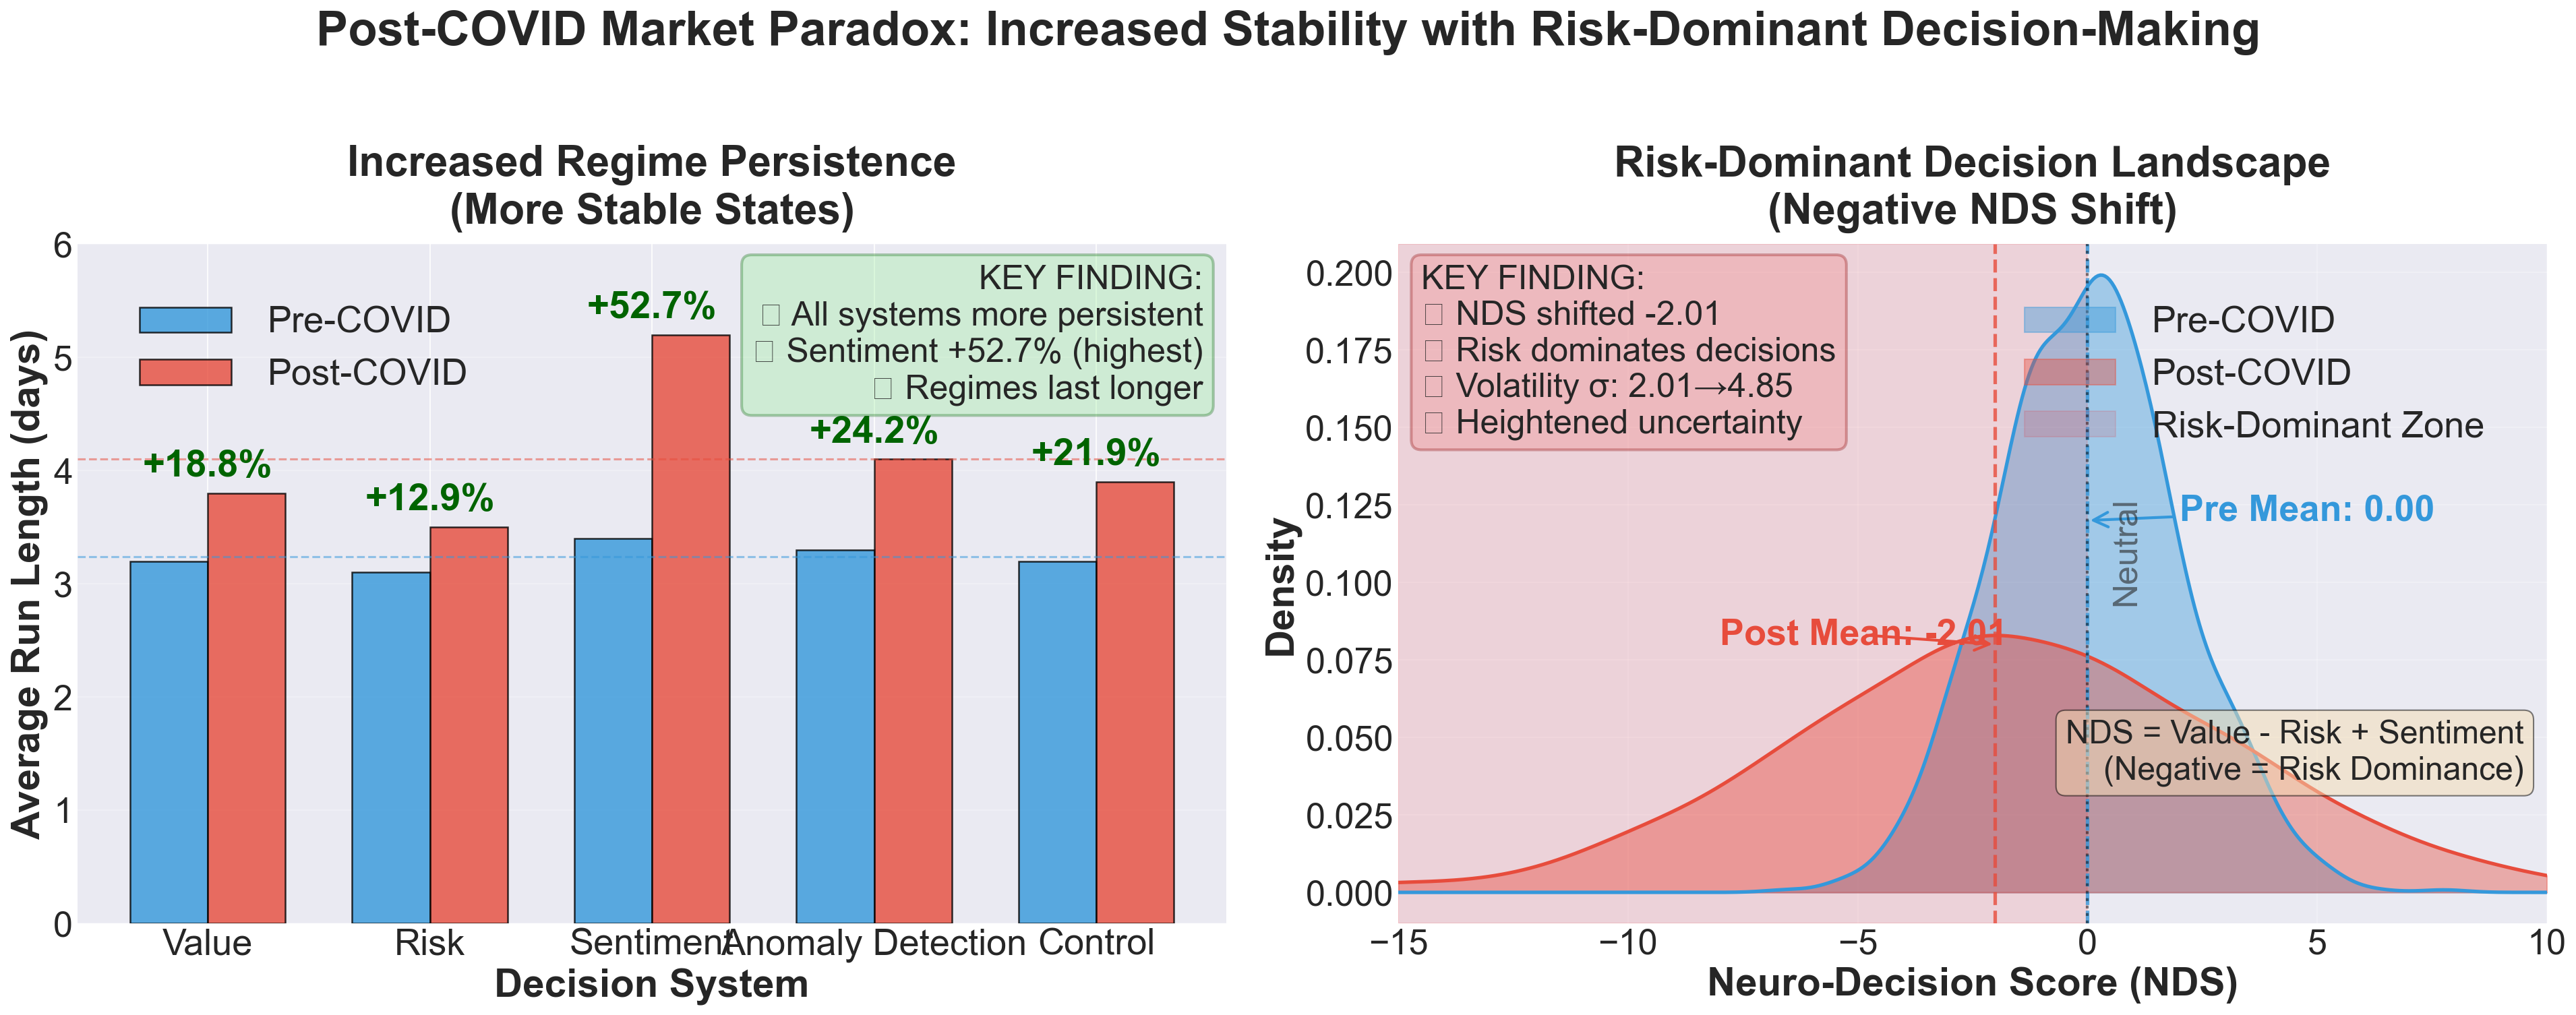
\includegraphics[width=0.7\textwidth]{stability_risk_paradox.png}
\caption{The Market Paradox. Post-COVID markets occupy the high-stability and high-risk quadrant.}
\label{fig:paradox}
\end{figure}

%------------------------------------------------------------------
\vspace{-15pt}
\section{Conclusion}

This study demonstrates that inferred market decision states using a machine learning model achieve classifier performance between 96--98\%. Longer persistence of market states is observed after COVID-19, with increased run lengths across systems, reflecting diminished flexibility and lower diversity in decision patterns. A transition into a new structural regime, rather than a temporary disruption, is thereby indicated. Practical applications in risk monitoring and strategy evaluation are enabled through the focus on latent decision dynamics rather than prices alone. The study focuses on the NIFTY Bank Index, with future extensions to broader indices such as NIFTY 50 to evaluate generalizability. The classifier achieved 96--98\% accuracy under the defined computational and validation framework described in Section~2.

%------------------------------------------------------------------
\vspace{-15pt}
\section*{Acknowledgment}
\vspace{-10pt}
The authors acknowledge the use of an LLM model for language editing assistance.

%------------------------------------------------------------------
\vspace{-15pt}
\begin{thebibliography}{15}

\bibitem{lo2004}
Lo, A.W.: The adaptive markets hypothesis. Journal of Portfolio Management \textbf{30}(5), 15--29 (2004)

\bibitem{hamilton1989}
Hamilton, J.D.: A new approach to the economic analysis of nonstationary time series and the business cycle. Econometrica \textbf{57}(2), 357--384 (1989)

\bibitem{shiller2021}
Shiller, R.J.: Narrative economics. American Economic Review \textbf{111}(4), 967--1004 (2021)

\bibitem{farmer2019}
Farmer, J.D., Gallegati, M., Hommes, C., et al.: A complex systems approach to constructing better models for managing financial markets and the economy. European Physical Journal Special Topics \textbf{214}, 295--324 (2019)

\bibitem{baker2020}
Baker, S.R., Bloom, N., Davis, S.J., Kost, K., Sammon, M., Viratyosin, T.: The unprecedented stock market reaction to COVID-19. Review of Asset Pricing Studies \textbf{10}(4), 742--758 (2020)

\bibitem{zaremba2021}
Zaremba, A., Kizys, R., Aharon, D.Y., Demir, E.: Infected markets: Novel coronavirus, government interventions, and stock return volatility around the globe. Finance Research Letters \textbf{35}, 101597 (2021)

\bibitem{glimcher2014}
Glimcher, P.W., Fehr, E. (eds.): Neuroeconomics: Decision Making and the Brain. Academic Press (2014)

\bibitem{bach2012}
Bach, D.R., Dolan, R.J.: Knowing how much you don't know: A neural organization of uncertainty estimates. Nature Reviews Neuroscience \textbf{13}, 572--586 (2012)

\bibitem{coates2012}
Coates, J.M.: The Hour Between Dog and Wolf: Risk-Taking, Gut Feelings and the Biology of Boom and Bust. Fourth Estate, London (2012)

\bibitem{kahneman1979}
Kahneman, D., Tversky, A.: Prospect theory: An analysis of decision under risk. Econometrica \textbf{47}(2), 263--291 (1979)

\bibitem{demartino2010}
De~Martino, B., Camerer, C.F., Adolphs, R.: Amygdala damage eliminates monetary loss aversion. Proceedings of the National Academy of Sciences of the USA \textbf{107}, 3788--3792 (2010)

\bibitem{boorman2009}
Boorman, E.D., Sallet, J.: Mean-variance or prospect theory? The nature of value representations in the human brain. Journal of Neuroscience \textbf{29}(22), 7945--7947 (2009)

\bibitem{alcaro2011}
Alcaro, A., Panksepp, J.: The seeking mind: Primal neuro-affective substrates for appetitive incentive states and their pathological dynamics in addictions and depression. Neuroscience \& Biobehavioral Reviews \textbf{35}(9), 1805--1820 (2011)

\bibitem{gu2020}
Gu, S., Kelly, B., Xiu, D.: Empirical asset pricing via machine learning. Review of Financial Studies \textbf{33}(5), 2223--2273 (2020)

\bibitem{chen2016}
Chen, T., Guestrin, C.: XGBoost: A scalable tree boosting system. In: Proceedings of the ACM SIGKDD International Conference on Knowledge Discovery and Data Mining, pp.~785--794 (2016)

\end{thebibliography}

\end{document}